\documentclass[spanish]{udpreport}
\usepackage[utf8]{inputenc}
\usepackage[spanish]{babel}
\graphicspath{{images/}}
\usepackage{graphicx}
\usepackage{multirow}
\usepackage{verbatim} 
\usepackage{upgreek} 

% Podemos establecer el logo de alguna entidad o dejar el de la UDP (defecto)
\setlogo{EITFI}

\title{Metodologia RUP}
\author{Christian López \\ Thomas Muñoz \\ Flavio Pallini}
\email{christian.lopeza@mail.udp.cl }
\date{29 de agosto de 2017}

% Además podemos establecer la facultad y escuela
% los valores por defecto son los siguientes:
\udpschool{Escuela de Informática y Telecomunicaciones}
\udpfaculty{Facultad de Ingeniería}
\udpuniversity{Universidad Diego Portales}

\begin{document}
\maketitle

\tableofcontents
\listoffigures
%\begin{figure}
%\centering
%\includegraphics[width=0.5\textwidth]{name_image.jpg}
%\caption{\label{fig:name}This is a figure caption.}
%\end{figure}

\chapter{Introducción}



\chapter{Explicación de Metodologia}

La metodologia RUP, es un proceso propietario por ingenieria de software creado por \textit{Rational Sowftware}, y actualmente propiedad de IBM, obteniendo el nombre de \textit{Rational Unified Process}, proporcionando tecnicas que deben seguir los miembro del equipo  de desarrolo de software. \par

Utiliza un enfoque de la orientacion a objecto en su diseño y documentado el uso de la notacion UML(\textit{Unified Modeling Languaje}) para ilustrar los procesos en acción. \par

\section{Por que utilizar RUP?}
\label{sec: Por que utilizar RUP}
RUP  le proporciona información sobre lo que puede esperarse de la tarea de desarrollo.Le ofrece un glosario de terminología y una enciclopedia de conocimiento que le ayuda a comunicar sus necesidades de formca eficaz al equipo de  desarrollo de software. \par
Para un gestór o jefe de equipo, RUP le proporciona  un proceso  el cual le permite comunicarse de forma eficaz con el personal y gestionar la planificación y el control de su trabajo. Para un Ingeniero en proceso, RUP le proporciona una buena base de arquitectura y una gran cantidad de materiales con las que construir una definicion de un proceso, lo que le permite configurar y ampliar dicha base como desee.

\section{Cuando debo utilizar RUP?}
\label{sec: Cuando debo utilizar RUP}
Se utiliza RUP desde el inicio de  un proyecyo de software, y puede seguir utilizándolo en los ciclos de desarrollo subsiguientes tiempo después de que le proyecto inicial haya terminado. \par
La forma de utilizar RUP varía para ajustarse a sus necesidades. Existen unas pocas consideraciones que determinarán cuando y como utilizar partes diferentes de RUP.
\begin{itemize}
\item Ciclo vital del proyecto(numero de iteraciones, longitud de cada fase)
\item Propósitos empresariales, visión, ámbito y riesgo del proyecto
\item Tamaño del esfuerzo de desarrollo de software
\end{itemize}
En la siguiente figura \ref{fig:grafico} muestra atraves de un grafico de complejidad de tecnica y gestion:

\begin{figure}[h]
	\centering
	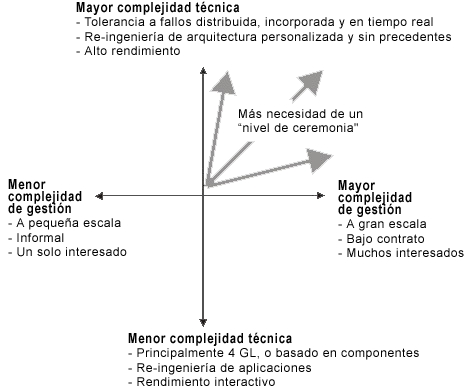
\includegraphics[width=0.7\textwidth]{RUP.png}
	\caption{\label{fig:grafico}Grafico complejidad de tecnica y gestion.}
\end{figure}

\section{Fases de la metodologia RUP}
Las fases indican el énfasis que se da en el proyecto en un instante dado. Para capturar la dimension temporal de un proyecto, RUP divide el proyecto en cuatro fases diferentes(ver figura \ref{fig:fases}):

\begin{figure}[!h]
	\centering
	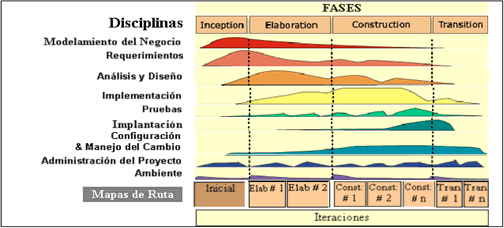
\includegraphics[width=0.8\textwidth]{fases.png}
	\caption{\label{fig:fases}Fases de RUP.}
\end{figure}

\begin{itemize}
\item Iniciación o Diseño: énfasis en el alcance del sistema
\item Preparación: énfasis en la arquitectura
\item Construcción: énfasis en el desarrollo
\item Transición: énfasis en la aplicacion

\end{itemize}

\subsection{Fase de Inicio}


\chapter{Aplicacion en Canchapp}

\chapter{Conclusion}


%\listoftables


\end{document}

